\documentclass[tikz,convert={outfile=free-cat-morphism.svg,density=1000}]{standalone}
\begin{document}
\tikzstyle{every node}=[font=\footnotesize]
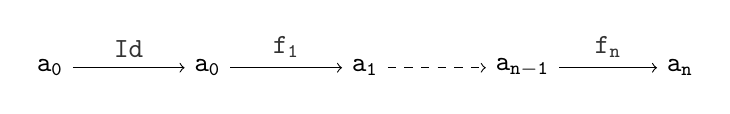
\begin{tikzpicture}
    \node (A) at (0,0) {\texttt{$\mathtt{a_0}$}};
    \node (B) at (2,0) {\texttt{$\mathtt{a_0}$}};
    \draw[->] (A) -- node[above] {\textcolor{black!80}{$\mathtt{Id}$}} (B);
    \node (C) at (4,0) {\texttt{$\mathtt{a_1}$}};
    \draw[->] (B) -- node [above] {\textcolor{black!80}{$\mathtt{f_1}$}} (C);
    \node (D) at (6,0) {\texttt{$\mathtt{a_{n-1}}$}};
    \draw[dashed,->] (C) -- (D);
    \node (E) at (8,0) {\texttt{$\mathtt{a_n}$}};
    \draw[->] (D) -- node [above] {\textcolor{black!80}{$\mathtt{f_n}$}} (E);
\end{tikzpicture}
\end{document}

